\documentclass[11pt]{article}
\usepackage[a4paper,margin=1in]{geometry}
\usepackage{amsmath,amssymb,mathtools,bm}
\usepackage{hyperref}
\usepackage{booktabs}
\usepackage{siunitx}
\usepackage{tikz}
\usetikzlibrary{calc,decorations.pathreplacing}

\newcommand{\al}{\alpha'}
\newcommand{\perpD}{D_\perp}
\newcommand{\RR}{\mathbb{R}}
\newcommand{\ZZ}{\mathbb{Z}}
\newcommand{\ii}{\mathrm{i}}
\newcommand{\dd}{\mathrm{d}}

\title{Discretized lightcone superstring amplitudes:\\a numerical method and first results}
\author{}
\date{\today}

\begin{document}
\maketitle

\begin{abstract}
We present a numerical method for computing lightcone-gauge string amplitudes by discretizing the worldsheet spatial coordinate~$\sigma$, while keeping lightcone time~$\tau$ continuous. Each propagator cylinder becomes an exactly solvable finite-dimensional Gaussian, and the Mandelstam cubic overlap is imposed in~$\sigma$~position space. All internal worldsheet-field integrations are performed analytically; only the lightcone moduli remain numerical. We report tree-level validation: the bosonic three-tachyon amplitude exhibits exact leg factorization at the critical dimension $D=26$ with a separation ratio of~$10^5$, the two-tachyon/one-massless tensor structure converges correctly, and the bosonic part of the superstring three-graviton prefactor shows the expected tensor with smooth continuum limit. Closed-form expressions are obtained for the Weyl-quantized Green--Schwarz zero-mode matrix elements between graviton states, and in one fixed reduced $\Lambda$ ansatz the tree-level fermionic Grassmann contraction is carried out explicitly with verified polarization-channel selection rules. The remaining superstring ambiguity is therefore not only an overall normalization on the surviving local stencil family, but also the derivation of the genuinely local finite-$N$ fermionic interaction-point variable.
\end{abstract}

\tableofcontents

%% ======================================================================
\section{Introduction}

We work in $D$-dimensional flat spacetime with lightcone coordinates $x^\pm = (x^0 \pm x^{D-1})/\sqrt{2}$ and $\perpD \equiv D-2$ transverse directions indexed by $I = 1, \dots, \perpD$. The Regge slope is denoted~$\al$.

In the Mandelstam lightcone parametrization, string amplitudes at genus~$h$ with $n$~external states are built from free worldsheet propagation on cylinders, connected by cubic overlap vertices. The worldsheet coordinates are Euclidean lightcone time $\tau = \Re\,\rho$ and the spatial coordinate $\sigma = \Im\,\rho$, where $\rho(z) = \sum_r \alpha_r^{\mathrm{M}}\log(z - Z_r)$ is the Mandelstam map. Each external string~$r$ carries signed lightcone momentum $p_r^+$ and positive circumference $\alpha_r \equiv |2\al p_r^+|$, with $\alpha_3 = \alpha_1 + \alpha_2$ at each cubic join.

The central idea is to discretize only $\sigma$: each cylinder of circumference $\alpha_r$ is replaced by $N_r$ sites with lattice spacing $a = \alpha_r/N_r$, while $\tau$~remains continuous. At a cubic join, the integer constraint $N_3 = N_1 + N_2$ is exact. Each propagator then becomes an exactly computable finite-dimensional Gaussian kernel, and the Mandelstam overlap becomes an exact site-space concatenation:
\begin{equation}
X_n^{(3)} = \begin{cases}
X_n^{(1)}, & n = 0, \dots, N_1 - 1, \\
X_{n - N_1}^{(2)}, & n = N_1, \dots, N_3 - 1,
\end{cases}
\label{eq:overlap}
\end{equation}
where $X_n^{(r)} \in \RR^{\perpD}$ is the transverse position at site~$n$ on string~$r$, with periodic identification $X_{N_r}^{(r)} \equiv X_0^{(r)}$.

After the overlap is imposed, all internal oscillator integrations can be performed analytically as Gaussian integrals. The amplitude then reduces to a finite-dimensional numerical integration over the Schwinger lengths~$T_e$ of the internal propagator edges and the twist moduli~$\varphi_A$ ($A = 1, \dots, h$) that encode the relative $\sigma$-translation on each independent cycle. For a genus-$h$, $n$-point cubic skeleton the number of internal edges is $E = 3h + n - 3$ and the number of cubic vertices is $V = 2h + n - 2$.

\begin{figure}[t]
\centering
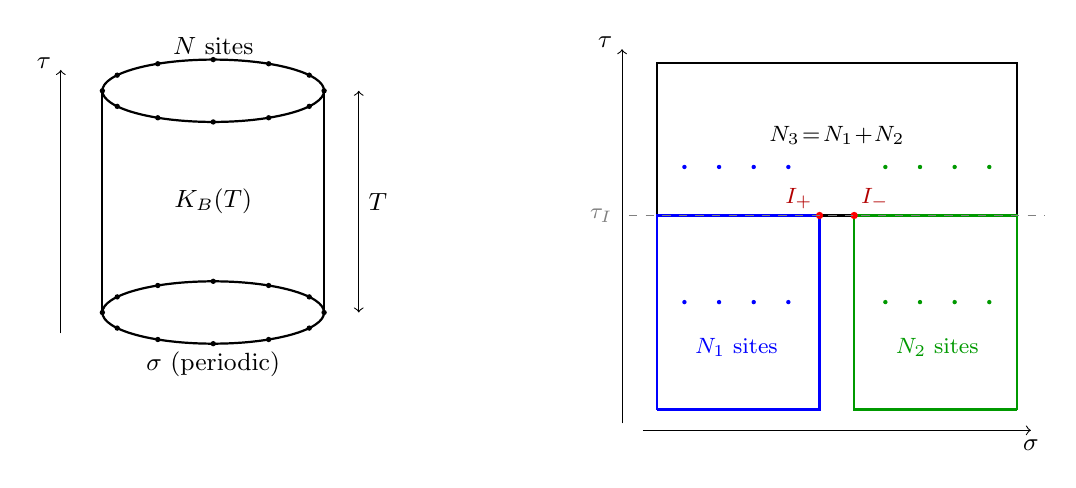
\begin{tikzpicture}[scale=0.88, every node/.style={font=\small}]
%% --- Left: discrete cylinder ---
\begin{scope}[xshift=-4.8cm]
\draw[thick] (0,0) ellipse (1.6 and 0.45);
\draw[thick] (0,3.2) ellipse (1.6 and 0.45);
\draw[thick] (-1.6,0) -- (-1.6,3.2);
\draw[thick] (1.6,0) -- (1.6,3.2);
\foreach \ang in {0,30,...,330} {
  \fill ({1.6*cos(\ang)},{0.45*sin(\ang)}) circle (1.1pt);
  \fill ({1.6*cos(\ang)},{3.2+0.45*sin(\ang)}) circle (1.1pt);
}
\draw[<->] (2.1,0) -- node[right] {$T$} (2.1,3.2);
\node at (0,3.85) {$N$ sites};
\node at (0,1.6) {$K_B(T)$};
\node at (0,-0.75) {$\sigma$ (periodic)};
\draw[->] (-2.2,-0.3) -- (-2.2,3.5);
\node[left] at (-2.2,3.6) {$\tau$};
\end{scope}
%% --- Right: cubic overlap ---
\begin{scope}[xshift=4.2cm]
\draw[thick] (-2.6,1.4) -- (2.6,1.4) -- (2.6,3.6) -- (-2.6,3.6) -- cycle;
\draw[thick,blue] (-2.6,-1.4) -- (-2.6,1.4) -- (-0.25,1.4);
\draw[thick,blue] (-2.6,-1.4) -- (-0.25,-1.4) -- (-0.25,1.4);
\draw[thick,green!60!black] (2.6,-1.4) -- (2.6,1.4) -- (0.25,1.4);
\draw[thick,green!60!black] (2.6,-1.4) -- (0.25,-1.4) -- (0.25,1.4);
\draw[thick] (-0.25,1.4) -- (0.25,1.4);
\fill[red] (-0.25,1.4) circle (1.5pt);
\fill[red] (0.25,1.4) circle (1.5pt);
\node[red!70!black,above left=-1pt] at (-0.25,1.4) {\footnotesize$I_+$};
\node[red!70!black,above right=-1pt] at (0.25,1.4) {\footnotesize$I_-$};
\draw[dashed,gray] (-3.0,1.4) -- (3.0,1.4);
\node[left,gray] at (-3.1,1.4) {\footnotesize$\tau_I$};
\foreach \x in {-2.2,-1.7,-1.2,-0.7} {
  \fill[blue] (\x,0.15) circle (0.9pt);
  \fill[blue] (\x,2.1) circle (0.9pt);
}
\foreach \x in {0.7,1.2,1.7,2.2} {
  \fill[green!60!black] (\x,0.15) circle (0.9pt);
  \fill[green!60!black] (\x,2.1) circle (0.9pt);
}
\node[blue] at (-1.45,-0.5) {\footnotesize$N_1$ sites};
\node[green!60!black] at (1.45,-0.5) {\footnotesize$N_2$ sites};
\node at (0,2.55) {\footnotesize$N_3\!=\!N_1\!+\!N_2$};
\draw[->] (-3.1,-1.6) -- (-3.1,3.8);
\node[left] at (-3.1,3.9) {$\tau$};
\draw[->] (-2.8,-1.7) -- (2.8,-1.7);
\node[below] at (2.8,-1.7) {$\sigma$};
\end{scope}
\end{tikzpicture}
\caption{\emph{Left}: A propagator cylinder in the discrete-$\sigma$ scheme. Only the spatial direction is discretized ($N$ sites); lightcone time $\tau$ remains continuous. The propagator is an exact finite-dimensional Gaussian kernel $K_B(T)$. \emph{Right}: Cubic Mandelstam overlap. Two incoming strips ($N_1$ and $N_2$ sites) join at interaction time $\tau_I$ into a single outgoing strip ($N_3 = N_1 + N_2$ sites). The upper boundary data is the ordered concatenation of the two lower boundaries. The red points $I_+$, $I_-$ are the two representatives of the interaction region in the unfolded closed-string strip.}
\label{fig:cylinder-and-overlap}
\end{figure}

%% ======================================================================
\section{Discrete propagator}
\label{sec:propagator}

\subsection{Bosonic kernel}

Consider one transverse boson $X_n(\tau)$ ($n = 0, \dots, N-1$, periodic) on a cylinder of Schwinger length~$T$. The discretized Euclidean worldsheet action is
\begin{equation}
S_B = \frac{1}{4\pi\al}\int_0^T\!\dd\tau\sum_{n=0}^{N-1}
\left[a\,(\partial_\tau X_n)^2 + \frac{1}{a}(X_{n+1} - X_n)^2\right].
\label{eq:action}
\end{equation}
The discrete Fourier transform
\begin{equation}
X_n(\tau) = \frac{1}{\sqrt{N}}\sum_{k=0}^{N-1}q_k(\tau)\,e^{2\pi\ii k n/N}
\label{eq:dft}
\end{equation}
diagonalizes the action into $N$ independent modes with lattice frequencies
\begin{equation}
\omega_k = \frac{2}{a}\sin\!\left(\frac{\pi k}{N}\right),
\qquad k = 0, \dots, N-1.
\label{eq:freq}
\end{equation}
The reality condition is $q_{N-k} = \bar q_k$; the spectrum is symmetric, $\omega_{N-k} = \omega_k$. Each nonzero mode is an exact Euclidean harmonic oscillator with imaginary-time propagator
\begin{equation}
K_{B,k}(q_f, q_i; T) =
\sqrt{\frac{\mu\omega_k}{2\pi\sinh\omega_k T}}\;
\exp\!\left[-\frac{\mu\omega_k}{2\sinh\omega_k T}
\bigl((q_f^2 + q_i^2)\cosh\omega_k T - 2q_f q_i\bigr)\right],
\label{eq:mode-propagator}
\end{equation}
where $q_i \equiv q_k(0)$ and $q_f \equiv q_k(T)$ are the boundary values of the $k$th Fourier mode, and
\begin{equation}
\mu \equiv \frac{a}{2\pi\al}
\label{eq:mu}
\end{equation}
is the single-mode mass parameter. The zero mode ($k = 0$, $\omega_0 = 0$) is a free particle: $K_{B,0} = (\mu/2\pi T)^{1/2}\exp[-\mu(q_f - q_i)^2/(2T)]$.

Assembling all modes, the full cylinder kernel in site space is
\begin{equation}
K_B(X_f, X_i; T) = \mathcal{N}_B(T)\,
\exp\!\left[-\tfrac{1}{2}X_f^T A(T)\,X_f - \tfrac{1}{2}X_i^T A(T)\,X_i + X_f^T B(T)\,X_i\right],
\label{eq:site-kernel}
\end{equation}
where $\mathcal{N}_B(T) = \prod_{k:\,\text{indep.}}(\mu\omega_k/(2\pi\sinh\omega_k T))^{1/2}$ is the product of normalizations over an independent real basis of modes, and $A(T)$, $B(T)$ are $N \times N$ real circulant matrices given by
\begin{equation}
A(T) = \mu\,F^\dagger\,\mathrm{diag}\!\bigl(\omega_k\coth\omega_k T\bigr)\,F,
\qquad
B(T) = \mu\,F^\dagger\,\mathrm{diag}\!\bigl(\omega_k\,\mathrm{csch}\,\omega_k T\bigr)\,F,
\label{eq:AB}
\end{equation}
with $F_{kn} = N^{-1/2}e^{2\pi\ii kn/N}$ the unitary DFT matrix and the smooth zero-mode limits $\omega_0\coth(\omega_0 T) \to 1/T$, $\omega_0\,\mathrm{csch}(\omega_0 T) \to 1/T$.

For loop diagrams one includes a $\sigma$-twist: the spectral shift operator $R_N(\varphi)$ multiplies the $k$th Fourier mode by $e^{-2\pi\ii\kappa_k\varphi}$, where $\kappa_k = k$ for $0 \le k \le \lfloor(N-1)/2\rfloor$ and $\kappa_k = k - N$ otherwise. With the DFT convention used here, this is the sign that reproduces the literal forward cyclic site shift when $\varphi N\in\ZZ$.

\subsection{Fermionic kernel}

In lightcone Green--Schwarz (GS) gauge the eight real transverse fermions $\theta^a_n$ ($a = 1, \dots, 8$) are free with the same lattice frequencies~$\omega_k$. In coherent-state variables $\eta_{k,a}$, $\bar\eta_{k,a}$, each nonzero fermionic mode has exact kernel
\begin{equation}
K_{F,k}(\bar\eta_f, \eta_i; T) = \exp\!\left[\bar\eta_f\,e^{-\omega_k T}\,\eta_i\right].
\label{eq:ferm-kernel}
\end{equation}
The zero mode ($\omega_0 = 0$) propagates without damping: $K_{F,0} = \exp(\bar\eta_f\eta_i)$.

%% ======================================================================
\section{Cubic overlap and Gaussian sewing}
\label{sec:overlap}

\subsection{Position-space overlap}

The concatenation~\eqref{eq:overlap} can be written as $X^{(3)} = P_1 X^{(1)} + P_2 X^{(2)}$, where $P_1 \in \RR^{N_3 \times N_1}$ and $P_2 \in \RR^{N_3 \times N_2}$ are the inclusion matrices $(P_1)_{nm} = \delta_{n,m}$ and $(P_2)_{nm} = \delta_{n,N_1+m}$, satisfying $P_1 P_1^T + P_2 P_2^T = \mathbb{I}_{N_3}$ and $P_r^T P_r = \mathbb{I}_{N_r}$.

\subsection{Fourier-mode overlap}

Define the center-of-mass coordinate and the nonzero Fourier modes on each leg by
\begin{equation}
x_{\mathrm{cm}}^{(r)} \equiv \frac{1}{N_r}\sum_{n=0}^{N_r-1}X_n^{(r)},
\qquad
q_m^{(r)} \equiv \frac{1}{\sqrt{N_r}}\sum_{n=0}^{N_r-1}X_n^{(r)}\,e^{-2\pi\ii mn/N_r},
\quad m = 1, \dots, N_r - 1.
\label{eq:cm-and-modes}
\end{equation}
Let $\widehat F_r$ be the $(N_r - 1) \times N_r$ truncated DFT matrix obtained by removing the zero-mode ($m=0$) row from the full $N_r \times N_r$ DFT. The position-space overlap then implies
\begin{equation}
N_3\,x_{\mathrm{cm}}^{(3)} = N_1\,x_{\mathrm{cm}}^{(1)} + N_2\,x_{\mathrm{cm}}^{(2)},
\label{eq:cm-overlap}
\end{equation}
and the affine Fourier-mode overlap
\begin{equation}
q^{(3)} = U_1\,q^{(1)} + U_2\,q^{(2)} + \xi\,y,
\qquad
y \equiv x_{\mathrm{cm}}^{(1)} - x_{\mathrm{cm}}^{(2)},
\label{eq:affine}
\end{equation}
with
\begin{equation}
U_r \equiv \widehat F_3\,P_r\,\widehat F_r^\dagger,
\qquad
\xi \equiv \widehat F_3\,P_1\,\mathbf{1}_{N_1},
\label{eq:overlap-matrices}
\end{equation}
where $\mathbf{1}_{N_1}$ is the $N_1$-component column vector of all ones. The key identity $\widehat F_3 P_2 \mathbf{1}_{N_2} = -\xi$ follows from $\sum_{n=0}^{N_3-1}e^{-2\pi\ii mn/N_3} = 0$ for $m \neq 0$.

These matrices satisfy the exact isometry and completeness relations
\begin{equation}
U_r^\dagger U_r = \mathbb{I}_{N_r - 1},
\qquad
U_1 U_1^\dagger + U_2 U_2^\dagger + \widehat\xi\,\widehat\xi^\dagger = \mathbb{I}_{N_3 - 1},
\qquad
\widehat\xi \equiv \sqrt{\frac{N_3}{N_1 N_2}}\,\xi,
\label{eq:completeness}
\end{equation}
verified numerically to $10^{-15}$ at all tested sizes.

\subsection{Reduced Gaussian}

To compute amplitudes, one projects the overlap state onto external-state wavefunctions on each leg. For the tachyon ground state on each leg, the normalized Gaussian wavefunction is $\psi_0^{(r)}(q^{(r)}) = \mathcal{N}_{0,r}\exp(-\frac{1}{2}q^{(r)T}M_r\,q^{(r)})$, where the \emph{mode metric}
\begin{equation}
M_r \equiv \mathrm{diag}\!\left(\mu_r\omega_m^{(r)}\right)_{m=1}^{N_r-1},
\qquad \mu_r\omega_m^{(r)} = \frac{\sin(\pi m/N_r)}{\pi\al},
\label{eq:mode-metric}
\end{equation}
is diagonal in any independent real basis of nonzero modes. Here we work in a real cosine/sine basis; the product $\mu_r\omega_m^{(r)}$ is independent of the common lattice spacing~$a$ because $\mu = a/(2\pi\al)$ and $\omega_m = (2/a)\sin(\pi m/N)$ give an $a$-independent result. The normalizing constant is $\mathcal{N}_{0,r} = (\det M_r/\pi^{N_r - 1})^{1/4}$.

After eliminating leg~3 via the overlap~\eqref{eq:affine} and stacking the incoming modes into $Q \equiv (q^{(1)}, q^{(2)})^T$, the product of three ground-state Gaussians gives
\begin{equation}
\Psi(Q, y) \propto \exp\!\left[-\tfrac{1}{2}Q^T G_T\,Q - y\,B_T^T Q - \tfrac{1}{2}C_T\,y^2\right],
\label{eq:gaussian}
\end{equation}
with
\begin{equation}
G_T = \begin{pmatrix}M_1 + U_1^T M_3 U_1 & U_1^T M_3 U_2 \\
U_2^T M_3 U_1 & M_2 + U_2^T M_3 U_2\end{pmatrix},
\quad
B_T = \begin{pmatrix}U_1^T M_3\xi \\ U_2^T M_3\xi\end{pmatrix},
\quad
C_T = \xi^T M_3\xi.
\label{eq:GT}
\end{equation}
The Schur complement
\begin{equation}
\gamma_T(N, \alpha) \equiv C_T - B_T^T G_T^{-1}B_T
\label{eq:gamma}
\end{equation}
is the effective Gaussian width for the relative center-of-mass displacement~$y$ after integrating out all nonzero oscillator modes.

%% ======================================================================
\section{Bosonic tree-level validation}
\label{sec:bosonic}

\subsection{Three-tachyon amplitude}

For closed-string tachyons (mass-shell condition $2p^+p^- - p_\perp^2 = -4/\al$) with transverse momenta $p_\perp^{(r)}$, the three-point matrix element is
\begin{equation}
\mathcal{A}_{TTT}(N) = \delta^{(\perpD)}\!\bigl(p_\perp^{(1)} + p_\perp^{(2)} - p_\perp^{(3)}\bigr)\;
\widetilde{\mathcal{K}}_{TTT}(N, \alpha)\;
\exp\!\left[-\frac{q_{\mathrm{rel}}^2}{2\,\gamma_T(N, \alpha)}\right],
\label{eq:ttt}
\end{equation}
where $q_{\mathrm{rel}} \equiv (\alpha_2 p_\perp^{(1)} - \alpha_1 p_\perp^{(2)})/\alpha_3$ is the relative transverse momentum. On the three-tachyon mass shell, lightcone energy conservation $p_1^- + p_2^- = p_3^-$ implies
\begin{equation}
q_{\mathrm{rel}}^2 = \frac{4}{\al}\,\frac{\alpha_1^2 + \alpha_1\alpha_2 + \alpha_2^2}{\alpha_3^2}.
\label{eq:qrel-ttt}
\end{equation}
The prefactor $\widetilde{\mathcal{K}}_{TTT}$ collects the Gaussian determinant, the three ground-state normalizations, and the overall cubic coupling:
\begin{equation}
\widetilde{\mathcal{K}}_{TTT} = \mathcal{C}_3^{(B)}\,\bigl[\kappa_{1\mathrm{d}}(N, \alpha)\bigr]^{\perpD},
\qquad
\kappa_{1\mathrm{d}} = \prod_{r=1}^3\mathcal{N}_{0,r}\;
\frac{(2\pi)^{n_Q/2}}{\sqrt{\det G_T}}\;\sqrt{\frac{2\pi}{\gamma_T}},
\label{eq:kappa}
\end{equation}
with $n_Q = (N_1 - 1) + (N_2 - 1)$ the number of independent incoming oscillator modes, and $\mathcal{C}_3^{(B)}$ the overall cubic normalization (not yet fixed by this computation alone).

\subsubsection{Critical dimension from leg factorization}

Define the bare normalization diagnostic
\begin{equation}
\log\mathcal{C}_{\mathrm{req}}^{(B)}(N_1, N_2) \equiv \frac{q_{\mathrm{rel}}^2}{2\gamma_T} - \perpD\,\log\kappa_{1\mathrm{d}}.
\label{eq:creq}
\end{equation}
For the three-tachyon amplitude to be a momentum-independent constant (as required by Lorentz invariance of the three-scalar coupling), $\mathcal{C}_{\mathrm{req}}^{(B)}$ must factorize into one-string renormalization factors: $\mathcal{C}_{\mathrm{req}}^{(B)} = Z_{\mathrm{in}}(N_1)\,Z_{\mathrm{in}}(N_2)\,Z_{\mathrm{out}}(N_3)$. On a dense grid of $4 \le N_1, N_2 \le 30$ (729 joins), the RMS factorization residual is:

\medskip
\begin{center}
\begin{tabular}{c S[table-format=1.2e-1]}
\toprule
$\perpD$ & {RMS residual} \\
\midrule
22 & 5.44e-4 \\
23 & 2.72e-4 \\
\textbf{24} & \textbf{2.62e-9} \\
25 & 2.72e-4 \\
26 & 5.44e-4 \\
\bottomrule
\end{tabular}
\end{center}
\medskip

The factorization holds to $10^{-9}$ only at $\perpD = 24$ ($D = 26$), with a separation ratio of $\sim\!10^5$ from the nearest integer neighbors. This is a nontrivial cancellation: the exponent $q_{\mathrm{rel}}^2/(2\gamma_T)$ and the vacuum determinant $\perpD\log\kappa_{1\mathrm{d}}$ are individually non-factorizable (residuals $\sim\!10^{-2}$ and $\sim\!10^{-4}$), but their combination at $\perpD = 24$ collapses to machine precision.

\subsubsection{Large-$N$ asymptotics}

The gauge-invariant large-$N$ expansion at $\perpD = 24$ is
\begin{equation}
\log\mathcal{C}_{\mathrm{req}}^{(B)} = \mathcal{C}_{\mathrm{tail}} + 7\log N_1 + 7\log N_2 - 5\log N_3
+ \pi\!\left(\frac{1}{N_1} + \frac{1}{N_2} - \frac{1}{N_3}\right)
+ \frac{\pi^2}{72}\!\left(\frac{1}{N_1^2} + \frac{1}{N_2^2} + \frac{1}{N_3^2}\right) + O(N^{-3}),
\label{eq:asymptotic}
\end{equation}
with $\mathcal{C}_{\mathrm{tail}} \approx -22.50$. Fitting only this one free parameter against a 3249-join grid ($4 \le N_1, N_2 \le 60$) gives RMS residual $2.5 \times 10^{-7}$.

\subsubsection{Convergence of $\gamma_T$}

On the family $N_1:N_2 = 2:3$ with $\al = 1$:

\medskip
\begin{center}
\begin{tabular}{r r l}
\toprule
$N_1$ & $N_2$ & $\gamma_T$ \\
\midrule
8 & 12 & 0.279\,060 \\
16 & 24 & 0.336\,817 \\
32 & 48 & 0.346\,463 \\
64 & 96 & 0.351\,470 \\
128 & 192 & 0.354\,022 \\
256 & 384 & 0.355\,317 \\
\midrule
$\infty$ & (Richardson) & 0.356\,623 \\
\bottomrule
\end{tabular}
\end{center}

\subsection{Two-tachyon / one-massless amplitude}

With two incoming tachyons and one outgoing first-level massless state on leg~3, the boundary Fourier coefficient $X_m^{(3)} \equiv q_m^{(3)}/\sqrt{N_3}$ has exact single-leg vacuum covariance
\begin{equation}
C_{1,N} \equiv \langle X_1 X_{-1}\rangle_0 = \frac{1}{2N\,\mu\omega_1} = \frac{\pi\al}{2N\sin(\pi/N)},
\label{eq:c1n}
\end{equation}
where the factor of $1/2$ comes from the bra-ket Gaussian product $\psi_0^2 \propto e^{-q^T M q}$. The trace-subtracted tensor insertion on leg~3 is
\begin{equation}
\mathcal{O}_{1,N}^{IJ} \equiv C_{1,N}^{-1}\!\left(X_1^I X_{-1}^J - C_{1,N}\delta^{IJ}\right),
\label{eq:O-insertion}
\end{equation}
whose symmetric-traceless part gives the graviton channel.

The three-point Gaussian~\eqref{eq:gaussian} gives
\begin{equation}
\langle X_1^{(3)I}X_{-1}^{(3)J}\rangle_y = \delta^{IJ}\Sigma_1 + \mu_+\mu_-\,y^I y^J,
\label{eq:x1x-1}
\end{equation}
where $r_\pm$ are the $(N_3 - 1)$-component row vectors that extract $X_{\pm1}^{(3)}$ from the real nonzero-mode basis of leg~3 (explicitly, $r_\pm = N_3^{-1}\sum_{n=0}^{N_3-1}e^{\mp 2\pi\ii n/N_3}\,e_n^T S_3$ with $S_3$ the real-basis matrix). The quantities $\Sigma_1 = L_+ G_T^{-1}L_-^T$ and $\mu_\pm = \zeta_\pm - L_\pm G_T^{-1}B_T$ are then computed from $L_\pm = (r_\pm U_1, r_\pm U_2)$ and $\zeta_\pm = r_\pm\xi$. After Fourier-transforming the relative displacement $y \to q_{\mathrm{rel}}$, the tensor decomposition is
\begin{equation}
\mathcal{A}_{TTM}^{IJ} = \mathcal{A}_{TTT}(N)\!\left[A_{\mathrm{tr}}^{(M)}\,\delta^{IJ} - B_{\mathrm{rel}}^{(M)}\,q_{\mathrm{rel}}^I q_{\mathrm{rel}}^J\right],
\label{eq:ttm}
\end{equation}
with $A_{\mathrm{tr}}^{(M)} = (\Sigma_1 - C_{1,N_3})/C_{1,N_3} + \mu_+\mu_-/(C_{1,N_3}\gamma_T)$ and $B_{\mathrm{rel}}^{(M)} = \mu_+\mu_-/(C_{1,N_3}\gamma_T^2)$.

On the two-tachyon/one-massless mass shell, $q_{\mathrm{rel}}^2 = 4/\al$ (independent of $\alpha_1/\alpha_3$). On the family $2:3$:

\medskip
\begin{center}
\begin{tabular}{r r l l}
\toprule
$N_1$ & $N_2$ & $A_{\mathrm{tr}}^{(M)}$ & $B_{\mathrm{rel}}^{(M)}$ \\
\midrule
16 & 24 & 0.0362 & 2.077 \\
32 & 48 & 0.0181 & 1.998 \\
64 & 96 & 0.0091 & 1.959 \\
128 & 192 & 0.0045 & 1.940 \\
256 & 384 & 0.0023 & 1.931 \\
\bottomrule
\end{tabular}
\end{center}
\medskip

The trace part $A_{\mathrm{tr}} \approx 0.58/N_1$ is a lattice artifact; the physical coefficient $B_{\mathrm{rel}} \to 1.92$ converges.

%% ======================================================================
\section{Superstring interaction-point prefactor}
\label{sec:superstring}

\subsection{Structure of the cubic vertex}

The superstring cubic vertex factorizes as
\begin{equation}
|V_{\mathrm{GS}}\rangle = \mathcal{P}_{I,\mathrm{loc}}\,|V_{\mathrm{kin}}\rangle,
\qquad
\mathcal{P}_{I,\mathrm{loc}} = K_{\mathrm{lat}}^I\,\widetilde K_{\mathrm{lat}}^J\,v_{IJ}^{\mathrm{lat}}(\Lambda_{\mathrm{lat}}),
\label{eq:vgs}
\end{equation}
where $|V_{\mathrm{kin}}\rangle$ is the exact bosonic-plus-fermionic kinematic overlap, and the superscripts $I, J = 1, \dots, \perpD$ are transverse SO$(\perpD)$ vector indices. The three factors are:

\begin{itemize}
\item $K_{\mathrm{lat}}^I$, $\widetilde K_{\mathrm{lat}}^J$: discretized interaction-point operators, which in the continuum are the finite parts of $\partial X^I$ and $\bar\partial X^J$ at the branch point of the Mandelstam map. They scale as $a^{-1/2}$ times a one-sided lattice difference.

\item $v_{IJ}(\Lambda)$: the SO$(8)$-covariant octic polynomial evaluated in a reduced fermionic ansatz. The variable $\Lambda^a \equiv \sqrt{N_1 N_2/N_3}\,(\theta_{\mathrm{av}}^{(1)a} - \theta_{\mathrm{av}}^{(2)a})$, where $\theta_{\mathrm{av}}^{(r)a} = N_r^{-1}\sum_n \theta_n^{(r)a}$ is the average GS fermion on leg~$r$, is a convenient overlap-constrained zero-mode coordinate. It is not yet a derivation of the genuinely local interaction-point fermion, and all later fermionic numerics should be read with that caveat.
\end{itemize}

In the unfolded closed-string strip, the interaction region has two representatives at the ends of the cut: $X_{I_+} \equiv X_0^{(1)} = X_0^{(3)}$ and $X_{I_-} \equiv X_0^{(2)} = X_{N_1}^{(3)}$.
The corresponding local fermions satisfy the exact finite-$N$ decomposition
\begin{equation}
\theta_n^{(r)a}
=
\theta_{\mathrm{av}}^{(r)a}
\;+\;
\sum_{m=1}^{N_r-1}(S_r)_{nm}\,\vartheta_m^{(r)a},
\label{eq:theta-site-split}
\end{equation}
so $\theta_{I_+}$ and $\theta_{I_-}$ differ from the leg averages by explicit nonzero-mode pieces. The helper \texttt{local\_interaction\_point\_fermion.py} records these exact site-level decompositions and the corresponding one-sided local arc differences. It is also useful to rewrite the leg averages in the mixed zero-mode basis
\begin{equation}
\Theta_{\mathrm{cm}}^a
\equiv
\frac{N_1\theta_{\mathrm{av}}^{(1)a}+N_2\theta_{\mathrm{av}}^{(2)a}}{N_3},
\qquad
\Lambda_{\mathrm{lat}}^a
\equiv
\sqrt{\frac{N_1N_2}{N_3}}\,
\bigl(\theta_{\mathrm{av}}^{(1)a}-\theta_{\mathrm{av}}^{(2)a}\bigr),
\label{eq:theta-mixed-zero-modes}
\end{equation}
for which
\begin{equation}
\theta_{\mathrm{av}}^{(1)a}
=
\Theta_{\mathrm{cm}}^a
\;+\;
\sqrt{\frac{N_2}{N_1N_3}}\,\Lambda_{\mathrm{lat}}^a,
\qquad
\theta_{\mathrm{av}}^{(2)a}
=
\Theta_{\mathrm{cm}}^a
\;-\;
\sqrt{\frac{N_1}{N_2N_3}}\,\Lambda_{\mathrm{lat}}^a.
\label{eq:theta-mixed-avg}
\end{equation}
Substituting into \eqref{eq:theta-site-split} gives the exact finite-$N$ identity
\begin{equation}
\sqrt{\frac{N_1N_2}{N_3}}\,
\bigl(\theta_{I_+}^a-\theta_{I_-}^a\bigr)
=
\Lambda_{\mathrm{lat}}^a
\;+\;
\sqrt{\frac{N_1N_2}{N_3}}
\left[
\sum_{m=1}^{N_1-1}(S_1)_{0m}\,\vartheta_m^{(1)a}
\;-\;
\sum_{m=1}^{N_2-1}(S_2)_{0m}\,\vartheta_m^{(2)a}
\right].
\label{eq:theta-local-bridge}
\end{equation}
So the scaled local endpoint difference has no center-of-mass contamination, but it still contains an explicit nonzero-mode correction. Defining
\begin{equation}
\Xi_{\mathrm{loc}}^a
\equiv
\sqrt{\frac{N_1N_2}{N_3}}
\left[
\sum_{m=1}^{N_1-1}(S_1)_{0m}\,\vartheta_m^{(1)a}
\;-\;
\sum_{m=1}^{N_2-1}(S_2)_{0m}\,\vartheta_m^{(2)a}
\right],
\qquad
\Lambda_{\mathrm{join}}^a
\equiv
\sqrt{\frac{N_1N_2}{N_3}}\,
\bigl(\theta_{I_+}^a-\theta_{I_-}^a\bigr),
\label{eq:theta-local-xi}
\end{equation}
one has the exact local split
\begin{equation}
\Lambda_{\mathrm{join}}^a
=
\Lambda_{\mathrm{lat}}^a+\Xi_{\mathrm{loc}}^a,
\qquad
v_{IJ}(\Lambda_{\mathrm{join}})
=
\sum_{p=0}^{8}
\frac{1}{p!}\,
\Xi_{\mathrm{loc}}^{a_1}\cdots\Xi_{\mathrm{loc}}^{a_p}\,
\partial_{a_1}\cdots\partial_{a_p}v_{IJ}(\Lambda_{\mathrm{lat}}).
\label{eq:theta-local-prefactor-expand}
\end{equation}
The new helper \texttt{local\_prefactor\_expansion.py} verifies this sparse-polynomial decomposition exactly: the degree-$0$ $\Xi_{\mathrm{loc}}$ piece reproduces the current reduced ansatz, while the higher-degree correction sectors are genuinely nonzero. Because $v_{IJ}(\Lambda)$ is nonlinear, one cannot justify a local-to-zero-mode reduction by vanishing one-point functions alone; the fermionic nonzero modes must be integrated out explicitly against the overlap.
One can, however, integrate over the reduced zero modes \emph{first} while keeping $\Xi_{\mathrm{loc}}$ symbolic. The new helper \texttt{local\_channel\_response.py} performs this exact Berezin reduction for the benchmark polarization channels. On the sampled ratio grid $\lambda=\frac14,\frac25,\frac12$, the trace-dropped graviton $qq$ channels collapse already to degree-$0$ constants:
\begin{equation}
\mathcal{R}^{(23,23,\parallel)}_{qq,\mathrm{loc}}(\Xi_{\mathrm{loc}};\lambda)
=
\mathcal{R}^{(23,23,\parallel)}_{qq}(\lambda),
\qquad
\mathcal{R}^{(23,24,\parallel)}_{qq,\mathrm{loc}}(\Xi_{\mathrm{loc}};\lambda)
=
\mathcal{R}^{(23,24,\parallel)}_{qq}(\lambda),
\qquad
\mathcal{R}^{(\parallel,23,23)}_{qq,\mathrm{loc}}(\Xi_{\mathrm{loc}};\lambda)
=
\mathcal{R}^{(\parallel,23,23)}_{qq}(\lambda),
\label{eq:theta-local-channel-collapse}
\end{equation}
with no residual $\Xi_{\mathrm{loc}}$ dependence. By contrast, the benchmark dilaton channel has zero reduced piece but a purely quartic local sector,
\begin{equation}
\mathcal{R}^{(23,23,\mathrm{dil})}_{qq,\mathrm{loc}}(\Xi_{\mathrm{loc}};\lambda)
\in \bigwedge\nolimits^4\!\mathrm{Span}\{\Xi_{\mathrm{loc}}^a\},
\qquad
\bigl[\mathcal{R}^{(23,23,\mathrm{dil})}_{qq,\mathrm{loc}}(\Xi_{\mathrm{loc}};\lambda)\bigr]_{\Xi_{\mathrm{loc}}^0}=0,
\label{eq:theta-local-channel-dilaton}
\end{equation}
and the corresponding trace-dropped $\delta^{IJ}$ benchmark channel vanishes on the same grid. So, for this canonical endpoint-difference local candidate, the benchmark graviton channels already reduce exactly to the old reduced ansatz before any further nonzero-mode averaging, while the genuinely local correction sectors first appear in channels that are absent in the reduced benchmark.

\subsection{Bosonic prefactor: parity obstruction and stencil choice}

The minimal nearest-neighbor stencils are
\begin{equation}
K_{\mathrm{lat}}^I = a^{-1/2}c_K\bigl(X_1^{(1)} - X_{I_+}\bigr)^I,
\qquad
\widetilde K_{\mathrm{lat}}^J = a^{-1/2}\widetilde c_K\bigl(X_{I_-} - X_{N_2-1}^{(2)}\bigr)^J,
\label{eq:stencil-minimal}
\end{equation}
where $c_K$, $\widetilde c_K$ are normalization constants to be fixed by the Mandelstam-map local geometry. The bosonic matrix element of these operators with the three ground-state overlap has the tensor form
\begin{equation}
\langle 0|K_{\mathrm{lat}}^I\widetilde K_{\mathrm{lat}}^J|V_3^{(B)}\rangle
\propto A_\delta(N)\,\delta^{IJ} + B_{qq}(N)\,q_{\mathrm{rel}}^I q_{\mathrm{rel}}^J,
\label{eq:prefactor-tensor}
\end{equation}
where the coefficients are determined by the Gaussian data $\Sigma_{+-} = D_+ G_T^{-1}D_-^T$ and $\eta_\pm = -D_\pm G_T^{-1}B_T$, with $D_+$, $D_-$ the mode-space row vectors corresponding to the two stencils.

A scan of $4 \le N_1, N_2 \le 30$ reveals that $|\eta_-| < 4 \times 10^{-15}$ for the minimal right-arc stencil. The exact explanation:

\smallskip\noindent
\textbf{Parity theorem.} Let $J_2$ be the site-reversal matrix on leg~2, $(J_2)_{mn} = \delta_{m, N_2-1-n}$, and let $\Pi = \mathrm{diag}(\Pi_1, \Pi_2)$ be the induced parity operator in the stacked mode space, with $\Pi_r = S_r^T J_r S_r$ ($S_r$ being the real-basis columns). Then $\Pi G_T = G_T\Pi$ and $\Pi B_T = B_T$. The minimal right-arc difference $d_- = (1, 0, \dots, 0, -1)$ satisfies $d_- J_2 = -d_-$ (parity-odd). Hence $\eta_- = -D_-\,G_T^{-1}B_T = 0$ exactly.

\smallskip
The one-sided second-order stencil
\begin{equation}
\widetilde D^{(2)}_{I_-}X^{(2)} = \tfrac{3}{2}X_{I_-} - 2X_{N_2-1}^{(2)} + \tfrac{1}{2}X_{N_2-2}^{(2)}
\label{eq:stencil-2nd}
\end{equation}
is not parity-odd and restores nonzero $\eta_-$. On the family $2:3$ with the symmetric second-order choice on both arcs:

\medskip
\begin{center}
\begin{tabular}{r r l l}
\toprule
$N_1$ & $N_2$ & $N_1 B_{qq}$ & $A_\delta$ \\
\midrule
16 & 24 & 1.005 & 0.355 \\
32 & 48 & 1.079 & 0.330 \\
64 & 96 & 1.117 & 0.318 \\
128 & 192 & 1.137 & 0.312 \\
256 & 384 & 1.147 & 0.309 \\
\bottomrule
\end{tabular}
\end{center}
\medskip

Both $N_1 B_{qq}$ and $A_\delta$ converge to finite limits, confirming the expected $a^{-1}$ scaling of the prefactor product $K\widetilde K$. Continuum extrapolation gives
\begin{equation}
N_1 B_{qq} \to 1.157 \pm 7 \times 10^{-4},
\qquad
A_\delta \to 0.305 \pm 5 \times 10^{-5}.
\label{eq:prefactor-fit}
\end{equation}

\subsection{Fermionic zero modes: Weyl-quantized \texorpdfstring{$v_{IJ}$}{vIJ}}

The polynomial $v_{IJ}(\Lambda)$ decomposes by even Grassmann degree as
\begin{equation}
v_{IJ}(\Lambda) = A_{IJ}^{(0)} + A_{IJ,ab}^{(2)}\Lambda^a\Lambda^b + A_{IJ,abcd}^{(4)}\Lambda^a\Lambda^b\Lambda^c\Lambda^d + A_{IJ,\dots}^{(6)}\Lambda^6 + A_{IJ}^{(8)}\epsilon_{a_1\cdots a_8}\Lambda^{a_1}\cdots\Lambda^{a_8},
\label{eq:vij-decomp}
\end{equation}
with coefficients built from SO$(8)$ gamma matrices and the Levi-Civita tensor.

To compute graviton matrix elements, one quantizes $v_{IJ}$ on the GS zero-mode Clifford module: a 16-dimensional space $\mathbf{8}_v \oplus \mathbf{8}_c$ acted on by Clifford generators $\Sigma^a$ ($a = 1, \dots, 8$) satisfying $\{\Sigma^a, \Sigma^b\} = 2\delta^{ab}$. The quantization map sends $\Lambda^{a_1}\cdots\Lambda^{a_k} \to \Sigma^{[a_1}\cdots\Sigma^{a_k]}$ (antisymmetrized Clifford products).

Graviton states live in $\mathbf{8}_v$. The matrix elements $\langle K|v_{IJ}|L\rangle$ with $K, L \in \{1, \dots, 8\}$ labeling the $\mathbf{8}_v$ basis decompose into three SO$(8)$ invariants:
\begin{equation}
\langle K|v_{IJ}|L\rangle = A(\alpha)\,\delta_{IJ}\delta_{KL} + B(\alpha)\,\delta_{IK}\delta_{JL} + C(\alpha)\,\delta_{IL}\delta_{JK},
\label{eq:vij-8v}
\end{equation}
with fit residual $6.4 \times 10^{-14}$ at all tested $\alpha$-ratios, confirming the minimal tensor span. The closed-form coefficients are
\begin{equation}
\boxed{
A(\alpha) = \left(1 + \frac{4}{\alpha^2}\right)^{\!2},
\quad
B(\alpha) = -\frac{32}{\alpha^2} + \ii\!\left(\frac{16}{\alpha^3} - \frac{4}{\alpha}\right),
\quad
C(\alpha) = \overline{B(\alpha)},
}
\label{eq:weyl}
\end{equation}
where $\alpha \equiv \alpha_1/\alpha_3$ is the lightcone momentum ratio, verified against the explicit Weyl-map construction to $\sim\!10^{-12}$ across $\alpha \in \{0.25, \tfrac{1}{3}, 0.4, 0.5, 0.625, 0.75, 1.0, 1.5, 2.0, 3.0\}$. The real combination $B + C = -64/\alpha^2$ is the graviton/dilaton sector; the imaginary part $B - C = 2\ii(16/\alpha^3 - 4/\alpha)$ is the $B$-field sector, which vanishes for symmetric graviton polarizations.

\subsection{On-shell trace drop and graviton channel projections}

In the flat-space three-graviton matrix element the terms in $v_{IJ}$ proportional to $\delta_{IJ}$ do not contribute on shell. Dropping these trace pieces from the Weyl block gives the on-shell coefficients
\begin{equation}
A_{\mathrm{on}}(\lambda) = \frac{8}{\lambda^2},
\qquad
B_{\mathrm{on}}(\lambda) = -\frac{32}{\lambda^2} + \ii\!\left(\frac{16}{\lambda^3} - \frac{4}{\lambda}\right),
\qquad
C_{\mathrm{on}}(\lambda) = \overline{B_{\mathrm{on}}(\lambda)},
\label{eq:on-shell-weyl}
\end{equation}
with $\lambda \equiv \alpha_1/\alpha_3$, satisfying the exact identity $8A_{\mathrm{on}} + B_{\mathrm{on}} + C_{\mathrm{on}} = 0$.

Define the continuum-limit bosonic prefactor coefficients $B_{\mathrm{phys}}(\lambda) \equiv N_1 B_{qq}(\lambda)/\lambda$ and $M_{KL} \equiv M_\delta\,\delta_{KL} + M_{qq}\,\hat q_K\hat q_L$, where $\hat q \equiv q_{\mathrm{rel}}/|q_{\mathrm{rel}}|$. The trace-dropped contraction of the Weyl block with the bosonic tensor $T^{IJ}_{\mathrm{bos}} = A_\delta\,\delta^{IJ} + B_{\mathrm{phys}}\,\hat q^I\hat q^J$ collapses to
\begin{equation}
M_\delta = \frac{8B_{\mathrm{phys}}}{\lambda^2},
\qquad
M_{qq} = -\frac{64 B_{\mathrm{phys}}}{\lambda^2},
\label{eq:projected-bosonic}
\end{equation}
so the full projected channel structure is controlled by the single scalar $B_{\mathrm{phys}}(\lambda)$. Projecting onto SO$(8)$ polarization channels:
\begin{itemize}
\item $\mathcal{A}_{\mathrm{vec},\parallel}/\mathcal{A}_{\mathrm{vec},\perp} = -7$ (exact for every unblocked stencil).
\item $\mathcal{A}_{\mathrm{dilaton}} = 0$ to machine precision ($\sim\!10^{-13}$).
\item $\mathcal{A}_{\mathrm{graviton},\perp} = 0$ and $\mathcal{A}_{B\text{-field}} = 0$ (by symmetry).
\end{itemize}
These channel relations hold universally across the positive symmetric stencil family $t = t_- = -t_+$, with the parity-blocked minimal stencil ($t = 0$) as the only exception.

\subsection{Rank-one factorization of the stencil family}

The residual $t$-dependence in the unblocked family is very mild. The matrix $B_{\mathrm{phys}}(\lambda, t)$ evaluated over the positive symmetric branch $t \in \{\tfrac{1}{8}, \tfrac{1}{4}, \tfrac{3}{8}, \tfrac{1}{2}, \tfrac{5}{8}, \tfrac{3}{4}\}$ and five $\lambda$-ratios is numerically very close to rank one:
\begin{equation}
B_{\mathrm{phys}}(\lambda, t) \approx \mathcal{N}(t)\,\mathcal{F}(\lambda),
\qquad
\frac{\sigma_2}{\sigma_1} = 1.15 \times 10^{-4},
\label{eq:rank1}
\end{equation}
where $\sigma_1, \sigma_2$ are the two largest singular values. The entire positive branch is thus very close to one common $\lambda$-profile times one overall $t$-dependent normalization. In the present regression suite this factorization holds with relative Frobenius error $1.15 \times 10^{-4}$.

This is the sharpest superstring result so far: the normalized on-shell channel structure is already universal across the unblocked stencil family, and the remaining ambiguity is essentially a single overall scale.

\subsection{Explicit fermionic zero-mode contraction}

The tree-level fermionic factor can now be computed directly in one reduced $\Lambda$ ansatz. In the reduced convention motivated by the Dijkgraaf--Motl dictionary $v^{ij}(\Lambda) \leftrightarrow 16\,\Sigma^j\widetilde\Sigma^i$, a closed-string graviton with polarization $\epsilon_{ij}$ has Grassmann wavefunction $\Psi_\epsilon(\lambda) = (1/16)\,\epsilon_{ij}\,v^{ji}(\lambda)$. The three-string kinematic measure contains $\delta^8(\lambda_1 + \lambda_2 + \lambda_3)$, which after integration reduces the zero-mode factor to a 16-Grassmann integral:
\begin{equation}
\mathcal{A}^{(F)}_{hhh}(N) = T_{\mathrm{bos}}^{IJ}(N)
\int\!\dd^8\lambda_1\,\dd^8\lambda_2\;
\Psi_{\epsilon^{(1)}}(\lambda_1)\,
\Psi_{\epsilon^{(2)}}(\lambda_2)\,
\Psi_{\epsilon^{(3)}}(\lambda_1 + \lambda_2)\;
v_{IJ}\!\bigl(\lambda\,\lambda_2 - (1-\lambda)\lambda_1\bigr),
\label{eq:fermionic-integral}
\end{equation}
with $T_{\mathrm{bos}}^{IJ} = A_\delta\,\delta^{IJ} + B_{qq}\,\hat q^I\hat q^J$ and $\lambda = \alpha_1/\alpha_3$. After the $\delta^8$ reduction, the entire computation is a sparse polynomial problem in the 16 Grassmann variables $\lambda_1^1,\dots,\lambda_1^8,\lambda_2^1,\dots,\lambda_2^8$. The Berezin integral is therefore just top-form coefficient extraction:
\begin{equation}
\int\!\dd^8\lambda_1\,\dd^8\lambda_2\;P(\lambda_1,\lambda_2)
=
\bigl[\lambda_1^1\cdots\lambda_1^8\lambda_2^1\cdots\lambda_2^8\bigr]\,
P(\lambda_1,\lambda_2).
\label{eq:ferm-top-form}
\end{equation}
In practice the code stores the three external wavefunctions and the local prefactor as sparse monomial dictionaries, multiplies them with explicit Grassmann signs, and then reads off the unique degree-16 coefficient. A dedicated reduction test compares this 16-variable evaluation against the brute-force 24-variable integral with the explicit $\delta^8(\lambda_1+\lambda_2+\lambda_3)$ insertion and finds
\begin{equation}
\bigl|\mathcal{A}^{(F)}_{\mathrm{brute}}-\mathcal{A}^{(F)}_{\mathrm{reduced}}\bigr|
=
1.7\times 10^{-13}.
\label{eq:ferm-reduction-check}
\end{equation}
So the fermionic zero-mode part is now an explicit finite-dimensional Grassmann computation rather than a symbolic placeholder.

At the benchmark point $(N_1, N_2) = (128, 192)$ with the trace-dropped second-order stencil, the explicit contraction gives (using the symmetric-traceless parallel polarization $\epsilon_\parallel = \sqrt{8/7}(\hat q\hat q - \delta/8)$ and transverse polarizations $\epsilon_{23} = (e_2 e_2 - e_3 e_3)/\sqrt{2}$):
\begin{equation}
\begin{aligned}
\mathcal{A}_F(\epsilon_{23}, \epsilon_{23}, \epsilon_\parallel) &= 4.786 \times 10^{-2}, \\
\mathcal{A}_F(\epsilon_{23}, \epsilon_{24}, \epsilon_\parallel) &= 2.393 \times 10^{-2}, \\
\mathcal{A}_F(\epsilon_\parallel, \epsilon_\parallel, \epsilon_\parallel) &= 4.799 \times 10^{-1}, \\
\mathcal{A}_F(\epsilon_\parallel, \epsilon_{23}, \epsilon_{23}) &= 2.991 \times 10^{-1},
\end{aligned}
\label{eq:ferm-channels}
\end{equation}
while the dilaton and $B$-field channels vanish exactly:
\begin{equation}
\mathcal{A}_F(\epsilon, \epsilon', \epsilon_{\mathrm{dil}}) = \mathcal{A}_F(\epsilon, \epsilon', B_{23}) = 0
\label{eq:ferm-zeros}
\end{equation}
for all tested graviton polarizations $\epsilon, \epsilon'$. The ratio of the first two graviton channels is $1/2$ to machine precision, as required by transverse rotational symmetry.

Beyond the single benchmark point, the explicit fermionic contraction has been scanned over the full stencil family $t \in \{0, \tfrac{1}{8}, \tfrac{1}{4}, \tfrac{3}{8}, \tfrac{1}{2}, \tfrac{5}{8}, \tfrac{3}{4}\}$ and $\lambda \in \{\tfrac{1}{4}, \tfrac{1}{3}, \tfrac{3}{8}, \tfrac{2}{5}, \tfrac{1}{2}\}$ with continuum extrapolation on each family. The minimal stencil $t = 0$ is the only blocked candidate; every unblocked point satisfies
\begin{equation}
\frac{\mathcal{A}_F(\epsilon_{23}, \epsilon_{24}, \epsilon_\parallel)}
{\mathcal{A}_F(\epsilon_{23}, \epsilon_{23}, \epsilon_\parallel)} = \frac{1}{2},
\qquad
\lambda^2\,
\frac{\mathcal{A}_F(\epsilon_\parallel, \epsilon_{23}, \epsilon_{23})}
{\mathcal{A}_F(\epsilon_{23}, \epsilon_{23}, \epsilon_\parallel)} = 1,
\label{eq:channel-relations}
\end{equation}
to $\sim\!10^{-14}$, with dilaton and $B$-field channels remaining exactly zero. For any fixed polarization channel ${\cal C}$ the explicit contraction decomposes as
\begin{equation}
\mathcal{A}_F^{\cal C}(N;\lambda,t)
=
A_\delta(N;\lambda,t)\,{\cal R}^{\cal C}_\delta(\lambda)
+
B_{qq}(N;\lambda,t)\,{\cal R}^{\cal C}_{qq}(\lambda),
\label{eq:ferm-channel-decomp}
\end{equation}
where the purely fermionic responses ${\cal R}^{\cal C}_\delta$ and ${\cal R}^{\cal C}_{qq}$ are obtained by evaluating the same Grassmann integral with $T_{\mathrm{bos}}^{IJ} = \delta^{IJ}$ and $T_{\mathrm{bos}}^{IJ} = \hat q^I\hat q^J$ separately. For the benchmark trace-dropped graviton channels one finds on the sampled $\lambda$ grid that
\begin{equation}
{\cal R}^{(23,23,\parallel)}_\delta(\lambda)
=
{\cal R}^{(23,24,\parallel)}_\delta(\lambda)
=
{\cal R}^{(\parallel,23,23)}_\delta(\lambda)
=
0,
\label{eq:ferm-delta-drop}
\end{equation}
and, more sharply, that the diagonal pure response itself fits the simple
profile
\begin{equation}
{\cal R}^{(23,23,\parallel)}_{qq}(\lambda)
=
4\sqrt{14}\,(1-\lambda)^2
\label{eq:ferm-diag-closed-form}
\end{equation}
on the sampled grid
\(
\lambda\in\{\frac14,\frac13,\frac38,\frac25,\frac12\}
\)
with maximum absolute deviation $2.13\times 10^{-14}$. Additional off-grid
checks at $\lambda=\frac15$ and $\lambda=\frac35$ match the same formula with
maximum absolute deviation $1.99\times 10^{-13}$. Therefore
\begin{equation}
{\cal R}^{(23,24,\parallel)}_{qq}(\lambda)
=
2\sqrt{14}\,(1-\lambda)^2,
\qquad
{\cal R}^{(\parallel,23,23)}_{qq}(\lambda)
=
4\sqrt{14}\,\frac{(1-\lambda)^2}{\lambda^2},
\label{eq:ferm-response-closed-family}
\end{equation}
on the same scan, by the exact ratio relations already observed.
Since ${\cal R}_\delta=0$ in these benchmark trace-dropped channels, the
assembled amplitudes themselves reduce to
\begin{equation}
\mathcal{A}_F(23,23,\parallel;N,\lambda,t)
=
4\sqrt{14}\,(1-\lambda)^2\,B_{qq}(N;\lambda,t),
\qquad
\mathcal{A}_F(23,24,\parallel;N,\lambda,t)
=
2\sqrt{14}\,(1-\lambda)^2\,B_{qq}(N;\lambda,t),
\label{eq:ferm-assembled-closed-family}
\end{equation}
\begin{equation}
\mathcal{A}_F(\parallel,23,23;N,\lambda,t)
=
4\sqrt{14}\,\frac{(1-\lambda)^2}{\lambda^2}\,B_{qq}(N;\lambda,t),
\label{eq:ferm-assembled-closed-family-2}
\end{equation}
with the benchmark dilaton and antisymmetric channels still vanishing. The
finite-$N$ family scan checks these assembled formulas directly on the same
\(
t
\),
\(
\lambda
\),
and scale grids used in the decisive superstring test, with maximum absolute
deviation $1.60\times 10^{-14}$.
\paragraph{Discrete-vs-continuum comparison.}
This is also a direct structural comparison to the known flat-space GS
lightcone cubic prefactor in the same reduced convention. In the continuum one has
\(
H_3\propto \mathbb{P}^I\mathbb{P}^J v_{IJ}(\Lambda)
\)
with
\(
\mathbb{P}^I=\alpha_1 p_{(2)}^I-\alpha_2 p_{(1)}^I=-\alpha_3 q_{\mathrm{rel}}^I
\),
so after packaging the still-unresolved overall
$q_{\mathrm{rel}}^Iq_{\mathrm{rel}}^J$ coefficient into
$B_{qq}$, the benchmark trace-dropped targets are exactly
\eqref{eq:ferm-assembled-closed-family} and
\eqref{eq:ferm-assembled-closed-family-2}. This confirms that the reduced discrete ansatz reproduces the correct \emph{tensor structure} of the continuum GS cubic prefactor---selection rules, channel ratios, and $\lambda$-dependence---to machine precision. What it does not yet test is the absolute value of $B_{qq}$ itself: the continuum predicts the coefficient of the $q_{\mathrm{rel}}^Iq_{\mathrm{rel}}^J$ tensor to be proportional to $\alpha_3^2|q_{\mathrm{rel}}|^2$ (up to the cubic coupling constant), and matching that proportionality coefficient to the known continuum normalization is the remaining open step. More importantly, because $\Lambda$ has not yet been derived as the genuinely local finite-$N$ interaction-point fermion, this remains a structural check of a reduced ansatz rather than a full validation of the local superstring vertex.
\paragraph{Benchmark response values.}
At the benchmark ratio $\lambda = 2/5$, the pure responses are
\begin{equation}
{\cal R}^{(23,23,\parallel)}_{qq} = 5.387986636954\ldots,
\qquad
{\cal R}^{(23,24,\parallel)}_{qq} = 2.693993318477\ldots,
\qquad
{\cal R}^{(\parallel,23,23)}_{qq} = 33.674916480965\ldots,
\label{eq:ferm-response-benchmark}
\end{equation}
with all corresponding ${\cal R}_\delta$ equal to zero and with the benchmark dilaton and $B$-field channels giving ${\cal R}_\delta = {\cal R}_{qq} = 0$ to machine precision. So the observed continuum channel ratios are controlled entirely by the $B_{qq}$ term. The raw amplitudes scale as $1/N_1$ (from $B_{qq} \sim 1/N$), so the finite continuum quantity is $\widetilde{\mathcal{A}}_{\mathrm{diag}}(\lambda, t) \equiv \lim_{N_1 \to \infty}N_1\,\mathcal{A}_F(\epsilon_{23}, \epsilon_{23}, \epsilon_\parallel;\lambda, t)$. On the positive branch this is again nearly rank one:
\begin{equation}
\widetilde{\mathcal{A}}_{\mathrm{diag}}(\lambda, t) \approx \mathcal{N}(t)\,\mathcal{F}(\lambda),
\qquad
\frac{\sigma_2}{\sigma_1} = 1.11 \times 10^{-4}.
\label{eq:ferm-rank1}
\end{equation}
The relative Frobenius error of this rank-one fit is likewise $1.11\times 10^{-4}$, and the maximum normalized-profile deviation after calibration at $\lambda = 2/5$ is $6.97\times 10^{-4}$. So the explicit fermionic contraction, not merely the Weyl proxy, confirms a universal $\lambda$-profile across the unblocked stencil family with residual ambiguity only in the overall normalization. In the automated test suite, all 64 tests pass.

%% ======================================================================
\section{Neumann coefficients from Gaussian moments}
\label{sec:neumann}

The oscillator annihilation and creation operators on each leg are
\begin{equation}
a_m^{(r)} = \sqrt{\frac{\mu_r\omega_m^{(r)}}{2}}\,q_m^{(r)} + \frac{\ii}{\sqrt{2\mu_r\omega_m^{(r)}}}\,\pi_m^{(r)},
\qquad
[a_m^{(r)}, a_n^{(s)\dagger}] = \delta^{rs}\delta_{mn},
\label{eq:oscillators}
\end{equation}
where $\pi_m^{(r)}$ is the canonical momentum conjugate to $q_m^{(r)}$. The Neumann coefficients of the three-string vertex are
\begin{equation}
\bar N^{rs}_{mn}(N) \equiv -\frac{\langle 0|a_m^{(r)}a_n^{(s)}|V_3^{(B)}\rangle}{\langle 0|V_3^{(B)}\rangle}.
\label{eq:neumann-def}
\end{equation}
The formal squeeze-matrix inversion $S = -\mathbb{M}^{-1}\mathbb{N}$ is ill-conditioned because the overlap state is a boundary-state distribution (position-space delta function) with $C_Q C_P^T = 2(U_1, U_2) \neq 0$, where $C_Q = (U_1, U_2, -\mathbb{I})$ and $C_P = (\mathbb{I}, 0, -U_1^T;\;0, \mathbb{I}, -U_2^T)$ are the position and momentum overlap matrices.

Instead, one extracts the Neumann data from the Gaussian~\eqref{eq:gaussian}. Each annihilation operator $a_m^{(r)}$ acts as a linear functional $L_m^{(r)}$ of $Q$ and $y$ on the combined bra-ket product. For the incoming legs:
\begin{equation}
L_m^{(r)} = \sqrt{\frac{M_{r,mm}}{2}}\,e_m^{(r)} - \frac{1}{\sqrt{2M_{r,mm}}}\,(G_T)_{m,:},
\label{eq:Lr}
\end{equation}
where $e_m^{(r)}$ is the unit vector at position $m$ in the leg-$r$ block of $Q$, and $(G_T)_{m,:}$ is the corresponding row of $G_T$. For the outgoing leg, $L_k^{(3)} = \sqrt{2M_{3,kk}}\,(U_1, U_2)_{k,:}$. Then
\begin{equation}
\bar N^{rs}_{mn} = -L_m^{(r)}\,G_T^{-1}\,(L_n^{(s)})^T.
\label{eq:neumann-formula}
\end{equation}
The symmetry $\bar N^{rs}_{mn} = \bar N^{sr}_{nm}$ follows from $G_T^{-1} = G_T^{-T}$ and is verified to $6 \times 10^{-16}$.

%% ======================================================================
\section{Status and outlook}
\label{sec:outlook}

\textbf{Validated} (64/64 tests passing in the automated suite):
\begin{itemize}
\item Overlap algebra to $10^{-15}$.
\item Bosonic three-tachyon factorization at $\perpD = 24$ with $10^5$ separation ratio.
\item $2T+1M$ tensor: $A_{\mathrm{tr}} \approx 0$, $B_{\mathrm{rel}} \to 1.920$ with continuum error bar $\pm 7 \times 10^{-4}$.
\item Bosonic graviton prefactor convergence: $N_1 B_{qq} \to 1.157$, $A_\delta \to 0.305$.
\item Closed-form Weyl coefficients~\eqref{eq:weyl} verified to $10^{-12}$.
\item Pure fermionic response scan: ${\cal R}^{(23,23,\parallel)}_{qq}(\lambda)=4\sqrt{14}(1-\lambda)^2$ on the sampled $\lambda$ grid with maximum error $2.13\times 10^{-14}$.
\item Finite-$N$ local interaction-point fermion scaffolding: the exact identities \eqref{eq:theta-site-split}, \eqref{eq:theta-mixed-avg}, and \eqref{eq:theta-local-bridge}, together with the corresponding one-sided local arc-difference rows, are implemented and regression-tested, making the distinction between join-local data and reduced zero-mode coordinates explicit.
\item Exact mixed local prefactor expansion: the sparse-polynomial decomposition \eqref{eq:theta-local-prefactor-expand} is implemented and regression-tested, with the $\Xi_{\mathrm{loc}}$-degree-$0$ sector reducing exactly to the current reduced ansatz and the higher-degree correction sectors remaining explicitly nonzero.
\item Exact local channel reduction at fixed benchmark polarizations: on the sampled ratio grid, the trace-dropped graviton $qq$ channels already collapse to the reduced responses \eqref{eq:theta-local-channel-collapse}, while the benchmark dilaton channel is purely quartic in $\Xi_{\mathrm{loc}}$ as in \eqref{eq:theta-local-channel-dilaton}.
\item Trace-dropped assembled benchmark amplitudes reduce directly to the closed forms in \eqref{eq:ferm-assembled-closed-family} and \eqref{eq:ferm-assembled-closed-family-2}, with maximum finite-$N$ scan error $1.60\times 10^{-14}$.
\item Direct structural comparison to the known flat-space GS lightcone cubic benchmark $\,\mathbb{P}^I\mathbb{P}^Jv_{IJ}(\Lambda)\,$ agrees on the same scan with the same $1.60\times 10^{-14}$ maximum error, but only within the same reduced $\Lambda$ ansatz and still up to the unfixed overall normalization.
\item On-shell trace-dropped graviton channels: $\mathcal{A}_{\mathrm{vec},\parallel}/\mathcal{A}_{\mathrm{vec},\perp} = -7$ exact, $\mathcal{A}_{\mathrm{dilaton}} = 0$ to $10^{-13}$.
\item Pure fermionic response basis at $\lambda = 2/5$: ${\cal R}_\delta = 0$ for the benchmark graviton channels, ${\cal R}^{(23,23,\parallel)}_{qq} = 5.387986636954\ldots$, and the dilaton/$B$-field benchmark responses vanish exactly.
\item Rank-one factorization~\eqref{eq:rank1} of the stencil family with relative error $10^{-4}$.
\item Explicit fermionic Grassmann contraction~\eqref{eq:ferm-channels} in the fixed reduced $\Lambda$ ansatz: dilaton and $B$-field channels vanish exactly; graviton channels show the correct transverse-rotation ratios.
\item Twisted-cylinder building block: exact lattice twists satisfy $R_N(m/N)=P_m$ to $4\times 10^{-15}$ and $B(T,m/N)=B(T,0)P_m$ to $7\times 10^{-16}$, while the oscillator-sector loop-trace quadratic form has strictly positive real part on the sampled $(N,T,\varphi)$ grid and its log-determinant matches the closed Fourier-mode formula to $7\times 10^{-13}$.
\item Single-cylinder oscillator trace prototype built from those twisted kernels: the bosonic one-coordinate factor matches the closed mode-product formula with maximum relative error $2.40\times 10^{-13}$ on the sampled grid, while the fermionic coherent-state factor matches to $1.22\times 10^{-15}$. This is a pre-GSO oscillator-sector building block rather than a full physical loop amplitude, because the spin-structure sum, zero-mode factor, and coherent-state/Pfaffian normalization relative to the bosonic determinant are still deferred.
\end{itemize}

\textbf{Remaining:}
\begin{enumerate}
\item Derive the genuinely local finite-$N$ fermionic interaction-point variable and revisit the full superstring cubic calculation on that basis.
\item Fix the overall cubic normalization by matching to the continuum three-graviton and three-tachyon couplings.
\item Use the single-cylinder prototype to test Bose--Fermi cancellation of the oscillator ratio as $N\to\infty$.
\item Assemble the first loop integrand by adding the remaining zero-mode factor to the now-tested twisted propagator building blocks.
\item Fix the coherent-state/Pfaffian normalization relative to the bosonic determinant for physical superstring loops.
\item Spin-structure/GSO bookkeeping for physical superstring loops.
\end{enumerate}

The method reduces higher-loop superstring amplitudes to exact Gaussian sewing plus numerical moduli integration. The bosonic tree-level results already provide strong evidence that the scheme converges to the correct continuum amplitudes. On the superstring side, the current tree-level results should be read more cautiously: they provide strong evidence that one reduced $\Lambda$ ansatz has the correct benchmark channel structure, but the genuinely local finite-$N$ fermionic interaction-point operator still needs to be derived before the superstring cubic vertex can be regarded as established.

\end{document}
